\documentclass[11pt]{article}

\usepackage[T1]{fontenc}
\usepackage{lmodern}
\usepackage{microtype}
\usepackage[margin=1in]{geometry}
\usepackage{amsmath,amssymb,amsthm,mathtools}
\usepackage{bm}
\usepackage{xcolor}
\usepackage{enumitem}
\usepackage{booktabs,tabularx,array}
\usepackage{tikz}
\usetikzlibrary{arrows.meta,positioning,decorations.pathreplacing,calc}
\usepackage[most]{tcolorbox}
\usepackage{fancyhdr}
\usepackage{hyperref}

\definecolor{navy}{HTML}{17365D}
\definecolor{teal}{HTML}{147D92}
\definecolor{lightblue}{HTML}{EEF5FA}
\definecolor{lightgray}{HTML}{F5F6F8}
\definecolor{darkgray}{HTML}{3B4048}
\definecolor{softgreen}{HTML}{EEF7F2}
\definecolor{greenframe}{HTML}{39735B}

\hypersetup{
  colorlinks=true,
  linkcolor=navy,
  citecolor=teal,
  urlcolor=teal,
  pdftitle={Conditional Mutual Information in CFT as a Quantum Markov Recovery Defect},
  pdfauthor={Technical note based on Longo--Xu, Petz, and recovery theory}
}

\pagestyle{fancy}
\fancyhf{}
\fancyhead[L]{\small\color{darkgray}CFT conditional mutual information}
\fancyhead[R]{\small\color{darkgray}Quantum Markov recovery}
\fancyfoot[C]{\small\thepage}
\renewcommand{\headrulewidth}{0.4pt}
\setlength{\headheight}{14pt}

\newtheoremstyle{accenttheorem}
  {8pt}{8pt}{\itshape}{}
  {\color{navy}\bfseries}{.}{0.5em}{}
\theoremstyle{accenttheorem}
\newtheorem{theorem}{Theorem}
\newtheorem{proposition}[theorem]{Proposition}
\newtheorem{corollary}[theorem]{Corollary}

\theoremstyle{definition}
\newtheorem{definition}[theorem]{Definition}
\newtheorem{remark}[theorem]{Remark}

\newcommand{\cA}{\mathcal{A}}
\newcommand{\cM}{\mathfrak{M}}
\newcommand{\cN}{\mathfrak{N}}
\newcommand{\cR}{\mathcal{R}}
\newcommand{\cE}{\mathcal{E}}
\newcommand{\id}{\operatorname{id}}
\newcommand{\Tr}{\operatorname{Tr}}
\newcommand{\RE}{D}
\newcommand{\MI}{F}
\newcommand{\CMI}{I}
\newcommand{\eps}{\varepsilon}
\newcommand{\dd}{\,\mathrm{d}}
\newcommand{\1}{\mathbf{1}}
\newcommand{\supp}{\operatorname{supp}}
\newcommand{\Ad}{\operatorname{Ad}}

\newtcolorbox{mainresult}{
  enhanced,
  colback=lightblue,
  colframe=navy,
  boxrule=0.8pt,
  arc=2mm,
  left=5mm,right=5mm,top=3.5mm,bottom=3.5mm,
  title={\bfseries Main conclusion},
  coltitle=white,
  colbacktitle=navy,
  attach boxed title to top left={xshift=4mm,yshift=-2mm}
}

\newtcolorbox{interpretationbox}{
  enhanced,
  colback=softgreen,
  colframe=greenframe,
  boxrule=0.7pt,
  arc=1.8mm,
  left=4.5mm,right=4.5mm,top=3mm,bottom=3mm,
  title={\bfseries Interpretation},
  coltitle=white,
  colbacktitle=greenframe
}

\newtcolorbox{caveatbox}{
  enhanced,
  colback=lightgray,
  colframe=darkgray!60,
  boxrule=0.6pt,
  arc=1.5mm,
  left=4mm,right=4mm,top=3mm,bottom=3mm,
  title={\bfseries Touching-limit caveat},
  coltitle=darkgray,
  colbacktitle=lightgray
}

\setlist[itemize]{leftmargin=1.5em,itemsep=2pt,topsep=4pt}
\setlist[enumerate]{leftmargin=1.7em,itemsep=3pt,topsep=4pt}
\setlength{\parindent}{0pt}
\setlength{\parskip}{5.5pt}
\allowdisplaybreaks
\emergencystretch=2em

\title{\vspace{-1.7cm}\color{navy}\bfseries
Conditional Mutual Information in CFT as a Quantum Markov Recovery Defect\\[0.35em]
\large From Longo--Xu finiteness to Petz and Faulkner--Hollands recovery}
\author{}
\date{}

\begin{document}
\maketitle
\vspace{-1.5em}

\begin{abstract}
For three adjacent intervals in the vacuum of a chiral conformal net, the formal expression
\(S(AB)+S(BC)-S(B)-S(ABC)\) cannot be interpreted as a subtraction of four type-III entropies.  Longo and Xu nevertheless obtain a finite conditional mutual information through Araki relative entropy and a controlled singular limit.  This note explains why their quantity is naturally a \emph{quantum Markov recovery defect}.  In finite dimensions, conditional mutual information is exactly the loss of relative entropy under the channel that discards \(C\).  Petz's equality theorem identifies zero loss with exact recovery, while Hayden--Jozsa--Petz--Winter describe the corresponding short quantum Markov chains.  The recovery theorems of Fawzi--Renner and of Junge--Renner--Sutter--Wilde--Winter quantify the approximate case, and the work of Faulkner--Hollands--Swingle--Wang extends the required result to arbitrary von Neumann algebras.  Applied to the Longo--Xu cross-ratio formula, this yields an explicit lower bound on recovery fidelity and shows that a long middle interval makes the CFT vacuum approximately Markovian.
\end{abstract}

\vspace{1.2em}
\begin{center}
\begin{tcolorbox}[
  width=0.88\textwidth,
  enhanced,
  colback=lightblue!62,
  colframe=navy,
  boxrule=0.7pt,
  arc=1.8mm,
  left=5mm,right=5mm,top=3.5mm,bottom=3.5mm
]
\centering
{\color{navy}\bfseries Core bridge}\par\vspace{0.45em}
\[
 \CMI_\eps
 =D_{\cM_\eps}(\omega_\eps\Vert\sigma_\eps)
  -D_{\cN_\eps}(\omega_\eps|_{\cN_\eps}\Vert
                  \sigma_\eps|_{\cN_\eps})
 \ge -2\log F_{\mathrm{rec}}.
\]
Longo--Xu compute the limiting defect,
\(
 \CMI_\omega(A:C\mid B)=-\frac r6\log\eta
\),
while Petz and Faulkner--Hollands turn it into the operational bound
\[
 F_{\mathrm{rec}}\ge\eta^{r/12}.
\]
\end{tcolorbox}
\end{center}
\clearpage

\begin{mainresult}
Let
\[
 A=(x_0,x_1),\qquad B=(x_1,x_2),\qquad C=(x_2,x_3),
 \qquad x_0<x_1<x_2<x_3,
\]
put \(a=x_1-x_0\), \(b=x_2-x_1\), \(c=x_3-x_2\), and define
\[
 \eta:=\frac{b(a+b+c)}{(a+b)(b+c)}
 =\frac{(x_2-x_1)(x_3-x_0)}{(x_2-x_0)(x_3-x_1)}\in(0,1).
\]
For the free chiral fermion net with \(r\) complex (Dirac) components (central charge \(c=r\)), and for the finite-index class controlled by Longo--Xu, the adjacent-interval conditional mutual information is
\[
 \CMI_\omega(A:C\mid B)=-\frac r6\log\eta.
\]
After introducing a collar of width \(\eps>0\), this is a genuine relative-entropy loss
\[
 \CMI_\eps
 =D_{\cM_\eps}(\omega_\eps\Vert\sigma_\eps)
  -D_{\cN_\eps}(\omega_\eps\Vert\sigma_\eps),
\]
so the universal modularly rotated Petz map gives a recovered state
\(\widetilde\omega_\eps\) satisfying
\[
 F_{\cM_\eps}(\omega_\eps,\widetilde\omega_\eps)
 \ge e^{-\CMI_\eps/2}.
\]
Consequently,
\[
 \boxed{\quad
 \liminf_{\eps\downarrow0}
 F_{\cM_\eps}(\omega_\eps,\widetilde\omega_\eps)
 \ge \eta^{r/12},
 \quad}
\]
and
\[
 \boxed{\quad
 \limsup_{\eps\downarrow0}
 \|\omega_\eps-\widetilde\omega_\eps\|
 \le 2\sqrt{1-\eta^{r/6}}.
 \quad}
\]
Thus the cross ratio is an operational measure of the failure of the vacuum to form an exact quantum Markov chain across \(A\)--\(B\)--\(C\).
\end{mainresult}

\section{Finite-dimensional starting point: CMI is lost distinguishability}

Let \(\rho_{ABC}\) be a density matrix and write
\[
 \CMI_\rho(A:C\mid B)
 :=S(AB)_\rho+S(BC)_\rho-S(B)_\rho-S(ABC)_\rho.
\]
Introduce the reference state
\[
 \sigma_{ABC}:=\rho_A\otimes\rho_{BC}
\]
and the channel \(\mathcal N=\Tr_C\), which forgets \(C\).  Since
\(\mathcal N(\sigma_{ABC})=\rho_A\otimes\rho_B\), a direct calculation gives
\begin{align}
 D(\rho_{ABC}\Vert\rho_A\otimes\rho_{BC})
 &=S(A)_\rho+S(BC)_\rho-S(ABC)_\rho,\label{eq:rel-1}\\
 D(\rho_{AB}\Vert\rho_A\otimes\rho_B)
 &=S(A)_\rho+S(B)_\rho-S(AB)_\rho.\label{eq:rel-2}
\end{align}
(The first equality requires \(\operatorname{supp}\rho_{ABC}\le\operatorname{supp}(\rho_A\otimes\rho_{BC})\), automatic for faithful states, so that the relative entropy is finite.)
Subtracting \eqref{eq:rel-2} from \eqref{eq:rel-1} yields
\begin{equation}\label{eq:cmi-dpi-defect}
 \boxed{
 \CMI_\rho(A:C\mid B)
 =D(\rho_{ABC}\Vert\sigma_{ABC})
  -D(\mathcal N\rho_{ABC}\Vert\mathcal N\sigma_{ABC}).
 }
\end{equation}
Thus strong subadditivity is the data-processing inequality for the pair
\((\rho_{ABC},\rho_A\otimes\rho_{BC})\).  Conditional mutual information measures exactly how much distinguishability is lost when \(C\) is discarded.

\begin{center}
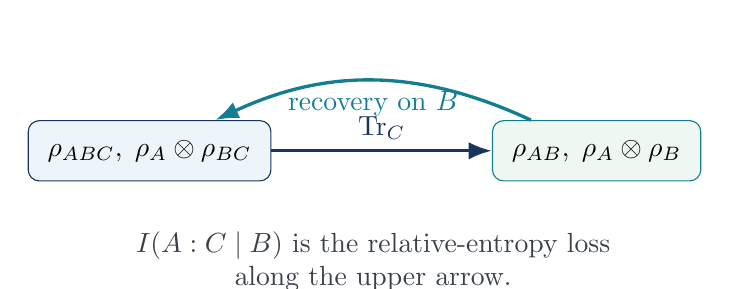
\begin{tikzpicture}[>=Latex,node distance=18mm and 28mm]
  \node[draw=navy,rounded corners,fill=lightblue,inner sep=7pt] (full)
    {$\rho_{ABC},\;\rho_A\otimes\rho_{BC}$};
  \node[draw=teal,rounded corners,fill=softgreen,inner sep=7pt,right=of full] (marg)
    {$\rho_{AB},\;\rho_A\otimes\rho_B$};
  \draw[->,very thick,navy] (full) -- node[above] {$\Tr_C$} (marg);
  \draw[<-,very thick,teal,bend left=25] (full) to node[below] {recovery on $B$} (marg);
  \node[below=9mm of $(full)!0.5!(marg)$,text=darkgray,align=center]
    {$\CMI(A:C\mid B)$ is the relative-entropy loss\\along the upper arrow.};
\end{tikzpicture}
\end{center}

\section{Petz equality and exact quantum Markov chains}

For a channel \(\mathcal N\) and a faithful reference state \(\sigma\), the Petz recovery map is
\begin{equation}\label{eq:general-petz}
 \cR^{\mathrm P}_{\sigma,\mathcal N}(X)
 =\sigma^{1/2}\,
   \mathcal N^*\!\left(
       \mathcal N(\sigma)^{-1/2}X\mathcal N(\sigma)^{-1/2}
   \right)\sigma^{1/2},
\end{equation}
with inverses taken on the relevant supports.  In the CMI setting, \eqref{eq:general-petz} factorizes as
\(\id_A\otimes\cR^{\mathrm P}_{B\to BC}\), where
\begin{equation}\label{eq:petz-B}
 \cR^{\mathrm P}_{B\to BC}(X_B)
 =\rho_{BC}^{1/2}
   \left(
      \rho_B^{-1/2}X_B\rho_B^{-1/2}\otimes\1_C
   \right)
   \rho_{BC}^{1/2}.
\end{equation}
(Here the Petz map is taken with respect to the reference state \(\sigma=\rho_A\otimes\rho_{BC}\) restricted to the subalgebra.)

Petz's equality theorem for relative entropy implies the following equivalence:
\begin{equation}\label{eq:markov-equivalence}
 \CMI_\rho(A:C\mid B)=0
 \quad\Longleftrightarrow\quad
 \rho_{ABC}
 =\bigl(\id_A\otimes\cR^{\mathrm P}_{B\to BC}\bigr)(\rho_{AB}).
\end{equation}
The right-hand side says that the full state can be reconstructed from \(AB\) by acting only on \(B\).  This is the defining property of a short quantum Markov chain
\[
 A\longleftrightarrow B\longleftrightarrow C.
\]

Hayden, Jozsa, Petz and Winter proved that, in finite dimensions, \eqref{eq:markov-equivalence} is also equivalent to a canonical decomposition of the middle Hilbert space,
\begin{equation}\label{eq:hjpw-decomposition}
 \mathcal H_B
 =\bigoplus_j \mathcal H_{b_j^L}\otimes\mathcal H_{b_j^R},
\end{equation}
for which
\begin{equation}\label{eq:hjpw-state}
 \rho_{ABC}
 =\bigoplus_j p_j\,
   \rho_{A b_j^L}\otimes\rho_{b_j^R C}.
\end{equation}
Conditioned on the classical label \(j\), the correlations with \(A\) and \(C\) occupy independent tensor factors of \(B\).

\begin{interpretationbox}
The Petz statement is the formulation that survives in quantum field theory.  The direct-sum tensor decomposition \eqref{eq:hjpw-decomposition} is tied to type-I algebras, whereas local CFT algebras are type III.  For type-III factors, exact Markovianity should be expressed as \emph{sufficiency of a von Neumann subalgebra}, or equivalently as exact Petz recovery.
\end{interpretationbox}

\section{The operator-algebraic Markov condition}

Let \(\cN\subset\cM\) be an inclusion of von Neumann algebras and let \(\rho,\sigma\) be faithful normal states on \(\cM\).  Define the data-processing defect
\begin{equation}\label{eq:abstract-defect}
 \delta_{\cN\subset\cM}(\rho,\sigma)
 :=D_{\cM}(\rho\Vert\sigma)
   -D_{\cN}(\rho|_{\cN}\Vert\sigma|_{\cN})\ge0.
\end{equation}
For faithful normal states with \(D_{\cM}(\rho\Vert\sigma)<\infty\), Petz's sufficiency theorem gives several equivalent characterizations of equality:
\begin{equation}\label{eq:petz-vn-equivalence}
 \delta_{\cN\subset\cM}(\rho,\sigma)=0
 \quad\Longleftrightarrow\quad
 \text{there is a normal unital 2-positive map $\alpha:\cM\to\cN$ with $\rho|_{\cN}\circ\alpha=\rho$ and $\sigma|_{\cN}\circ\alpha=\sigma$}.
\end{equation}
For faithful states, another equivalent condition is the Connes-cocycle criterion
\begin{equation}\label{eq:connes-criterion}
 [D\rho:D\sigma]_t\in\cN
 \qquad\text{for every }t\in\mathbb R.
\end{equation}
This is an intrinsically type-III replacement for density-matrix logarithm identities.  It makes the Markov property a statement about relative modular flow rather than about a Hilbert-space factorization.

\section{Collar regularization for three adjacent CFT intervals}

Let \(\cA(I)\) denote the local algebra of a chiral conformal net in the vacuum state \(\omega\).  Shorten the left interval by a collar,
\[
 A_\eps=(x_0,x_1-\eps),\qquad 0<\eps<a,
\]
while keeping
\(B=(x_1,x_2)\) and \(C=(x_2,x_3)\).  Define
\begin{equation}\label{eq:MN-def}
 \cM_\eps:=\cA(A_\eps)\vee\cA(BC),
 \qquad
 \cN_\eps:=\cA(A_\eps)\vee\cA(B),
 \qquad
 \cN_\eps\subset\cM_\eps.
\end{equation}
The split property of the free fermion net (Longo--Xu, Lemma~3.1 and the references there) identifies these algebras with the graded tensor products
\begin{equation}\label{eq:split-identification}
 \cM_\eps\simeq
 \cA(A_\eps)\,\overline\otimes\,\cA(BC),
 \qquad
 \cN_\eps\simeq
 \cA(A_\eps)\,\overline\otimes\,\cA(B).
\end{equation}
On \(\cM_\eps\), introduce the split reference state
\begin{equation}\label{eq:split-reference}
 \sigma_\eps:=\omega_{A_\eps}\otimes_2\omega_{BC},
\end{equation}
the graded product of Longo--Xu Lemma~3.1: it is the unique normal state on \(\cM_\eps\) with \(\sigma_\eps(xy)=\omega(x)\omega(y)\) for \(x\in\cA(A_\eps)\), \(y\in\cA(BC)\), it is faithful, and because \(\omega\) vanishes on odd elements the relative entropies below take the same values for the graded and the ordinary product notation (verification document \texttt{rigor/check\_notes\_1\_2.tex}).  Its restriction to \(\cN_\eps\) is
\[
 \sigma_\eps|_{\cN_\eps}=\omega_{A_\eps}\otimes\omega_B.
\]
Writing \(\omega_\eps:=\omega|_{\cM_\eps}\), the two relative entropies are precisely the Longo--Xu mutual informations,
\begin{align}
 D_{\cM_\eps}(\omega_\eps\Vert\sigma_\eps)
 &=\MI(A_\eps,BC),\label{eq:MI-big}\\
 D_{\cN_\eps}(\omega_\eps|_{\cN_\eps}\Vert\sigma_\eps|_{\cN_\eps})
 &=\MI(A_\eps,B).\label{eq:MI-small}
\end{align}
Therefore
\begin{equation}\label{eq:Ieps-defect}
 \boxed{
 \CMI_\eps(A:C\mid B)
 =\MI(A_\eps,BC)-\MI(A_\eps,B)
 =\delta_{\cN_\eps\subset\cM_\eps}(\omega_\eps,\sigma_\eps).
 }
\end{equation}
This is the exact operator-algebraic counterpart of \eqref{eq:cmi-dpi-defect}.

For the free \(r\)-fermion net, the separated-interval formula gives, in fact,
\begin{equation}\label{eq:Ieps-free}
 \CMI_\eps(A:C\mid B)
 =\frac r6\log\!\left[
   \frac{(a+b)(b+c+\eps)}{(a+b+c)(b+\eps)}
 \right].
\end{equation}
Taking \(\eps\downarrow0\), or using the Longo--Xu generalized mutual information for the overlapping intervals \(AB\) and \(BC\), gives
\begin{equation}\label{eq:longoxu-limit}
 \CMI_\omega(A:C\mid B)
 =\lim_{\eps\downarrow0}\CMI_\eps(A:C\mid B)
 =\frac r6\log\!\left[
   \frac{(a+b)(b+c)}{b(a+b+c)}
 \right]
 =-\frac r6\log\eta.
\end{equation}
For the finite-index subnets and extensions covered by Longo--Xu, the same balanced limit follows because the universal short-distance and index terms cancel in the relative-entropy difference.

\section{Faulkner--Hollands recovery for type-III algebras}

The finite-dimensional Fawzi--Renner theorem shows that small CMI implies good recovery.  The universal rotated-Petz constructions of Sutter--Fawzi--Renner and Junge--Renner--Sutter--Wilde--Winter make the recovery independent of the state being reconstructed.  Faulkner, Hollands, Swingle and Wang prove the corresponding strengthened data-processing inequality for arbitrary von Neumann subalgebras, precisely the setting needed for local CFT factors.

For a faithful reference state \(\sigma\) and an inclusion \(\cN\subset\cM\), let
\(\alpha_{\sigma,0}:\cM\to\cN\) be the Petz generalized conditional expectation.  In standard forms it may be written
\begin{equation}\label{eq:standard-petz}
 \alpha_{\sigma,0}(x)
 =J_{\cN}V_\sigma^*J_{\cM}\,x\,J_{\cM}V_\sigma J_{\cN},
\end{equation}
where \(V_\sigma\) is the canonical isometry implementing the inclusion.  Its modular rotations are
\begin{equation}\label{eq:rotated-petz}
 \alpha_{\sigma,t}
 =\sigma_{-t}^{\sigma|_{\cN},\cN}
  \circ\alpha_{\sigma,0}
  \circ\sigma_t^{\sigma,\cM},
 \qquad t\in\mathbb R,
\end{equation}
where \(\sigma_t^{\sigma,\cM}\) denotes the modular automorphism group.  Define the universal averaged channel
\begin{equation}\label{eq:averaged-petz}
 \overline\alpha_\sigma(x)
 :=\int_{-\infty}^{\infty}
    p(t)\,\alpha_{\sigma,t}(x)\dd t,
 \qquad
 p(t):=\frac{\pi}{1+\cosh(2\pi t)}.
\end{equation}
The kernel is normalized, \(\int_{\mathbb R}p(t)\dd t=1\).

The strengthened data-processing inequality of Faulkner--Hollands--Swingle--Wang (Theorem~1, eq.~(24)) is the integrated form \(D_{\cM}(\rho\Vert\sigma)-D_{\cN}(\rho|_{\cN}\Vert\sigma|_{\cN})\ge-2\int p(t)\log F_{\cM}(\rho,\rho|_{\cN}\circ\alpha_{\sigma,t})\,dt\) for normal \(\rho\) and faithful normal \(\sigma\); by concavity of the root fidelity it implies the averaged form (Faulkner--Hollands II, Theorem~2, eq.~(21)) used here, namely that
\begin{equation}\label{eq:FH-bound}
 D_{\cM}(\rho\Vert\sigma)
 -D_{\cN}(\rho|_{\cN}\Vert\sigma|_{\cN})
 \ge
 -2\log F_{\cM}\!\left(
   \rho,\rho|_{\cN}\circ\overline\alpha_\sigma
 \right).
\end{equation}
Consequently, if
\(\tilde\rho:=\rho|_{\cN}\circ\overline\alpha_\sigma\), then
\begin{align}
 F_{\cM}(\rho,\tilde\rho)
 &\ge e^{-\delta_{\cN\subset\cM}(\rho,\sigma)/2},
 \label{eq:fidelity-general}\\
 \|\rho-\tilde\rho\|
 &\le 2\sqrt{1-e^{-\delta_{\cN\subset\cM}(\rho,\sigma)}}.
 \label{eq:norm-general}
\end{align}
This is Theorem~2 of \cite{FHSW}.
The second estimate follows from the fidelity--norm inequalities for normal states.

In the CFT application, the product form \eqref{eq:split-reference} and the tensor-product inclusion \eqref{eq:split-identification} imply
\begin{equation}\label{eq:factorization-heisenberg}
 \overline\alpha_{\sigma_\eps}
 =\id_{\cA(A_\eps)}\,\overline\otimes\,
   \overline\alpha_{B\subset BC}.
\end{equation}
Thus, in the Schrodinger picture, the nontrivial recovery operation reconstructs \(BC\) from \(B\) and acts trivially on \(A_\eps\):
\begin{equation}\label{eq:factorization-schrodinger}
 \overline\cR_\eps
 =\id_{A_\eps}\,\overline\otimes\,
   \overline\cR_{B\to BC}.
\end{equation}
This is exactly the locality condition required of a quantum Markov chain.  (For the graded tensor product the factorization is proved with the Klein transformation; see Note~4, Lemma~3.1, and the verification documents.)

\section{Explicit CFT recovery bounds}

Apply \eqref{eq:FH-bound} to
\((\cN_\eps\subset\cM_\eps,\omega_\eps,\sigma_\eps)\) and define
\begin{equation}\label{eq:recovered-vacuum}
 \widetilde\omega_\eps
 :=\omega_\eps|_{\cN_\eps}
   \circ\overline\alpha_{\sigma_\eps}.
\end{equation}
Equations \eqref{eq:Ieps-defect} and \eqref{eq:fidelity-general} give
\begin{equation}\label{eq:eps-recovery-bound}
 F_{\cM_\eps}(\omega_\eps,\widetilde\omega_\eps)
 \ge e^{-\CMI_\eps(A:C\mid B)/2}.
\end{equation}
Using the Longo--Xu limit \eqref{eq:longoxu-limit},
\begin{equation}\label{eq:cross-ratio-fidelity}
 \liminf_{\eps\downarrow0}
 F_{\cM_\eps}(\omega_\eps,\widetilde\omega_\eps)
 \ge
 \exp\!\left[-\frac12\CMI_\omega(A:C\mid B)\right]
 =\eta^{r/12}.
\end{equation}
Likewise,
\begin{equation}\label{eq:cross-ratio-norm}
 \limsup_{\eps\downarrow0}
 \|\omega_\eps-\widetilde\omega_\eps\|
 \le2\sqrt{1-\eta^{r/6}}.
\end{equation}

\subsection{Exact versus approximate Markovianity}

For nondegenerate intervals \(a,b,c>0\),
\[
 \frac{(a+b)(b+c)}{b(a+b+c)}
 =1+\frac{ac}{b(a+b+c)}>1.
\]
Hence
\begin{equation}\label{eq:strict-positive}
 \CMI_\omega(A:C\mid B)>0.
\end{equation}
The vacuum is therefore not an exact quantum Markov chain in the collar-regularized Petz-sufficiency sense.  Nevertheless, it becomes approximately Markovian when the middle interval is long.  With \(a,c\) fixed and \(b\to\infty\),
\begin{equation}\label{eq:large-b-cmi}
 \CMI_\omega(A:C\mid B)
 =\frac r6\frac{ac}{b^2}+O(b^{-3}).
\end{equation}
The recovery estimates become
\begin{align}
 F_{\mathrm{rec}}
 &\ge1-\frac{r\,ac}{12b^2}+O(b^{-3}),
 \label{eq:large-b-fidelity}\\
 \|\omega-\widetilde\omega\|
 &\lesssim\frac{2}{b}\sqrt{\frac{r\,ac}{6}}.
 \label{eq:large-b-norm}
\end{align}
Thus the Markov defect decays algebraically rather than exponentially.  This is consistent with scale invariance: a CFT has no intrinsic finite correlation or Markov length.

\begin{center}
\small
\renewcommand{\arraystretch}{1.32}
\begin{tabularx}{0.91\textwidth}{>{\bfseries}p{0.17\textwidth} X}
\toprule
Regime & Markov and CFT interpretation \\
\midrule
\(\CMI=0\) & Exact Petz recovery and the HJPW short-Markov-chain structure.  This is not realized by three nondegenerate finite spatial intervals in the present vacuum geometry. \\
\(0<\CMI\ll1\) & High-fidelity recovery from \(AB\) by acting only on \(B\).  A long shielding interval gives \(\CMI\sim b^{-2}\). \\
\(0<\CMI<\infty\) & A nonzero universal recovery guarantee for every finite Longo--Xu cross ratio \(0<\eta<1\). \\
\bottomrule
\end{tabularx}
\end{center}

\section{What is and is not proved at zero collar width}

\begin{caveatbox}
For every \(\eps>0\), the split product state is normal, the algebras in \eqref{eq:split-identification} are genuine tensor products, and the Faulkner--Hollands theorem applies directly.  At \(\eps=0\), adjacent local algebras do not generally admit a normal product state.  Therefore the limit of the recovery \emph{bounds} does not by itself produce a single normal channel on the touching algebra.
\end{caveatbox}

What follows rigorously without an additional extension theorem is a family of collar-regularized recovery statements with a uniform limiting estimate, namely \eqref{eq:cross-ratio-fidelity}.  A natural route to a genuine touching-interval recovery map is suggested by \eqref{eq:factorization-heisenberg}: the nontrivial component
\[
 \overline\alpha_{B\subset BC}:\cA(BC)\longrightarrow\cA(B)
\]
depends only on the inclusion \(\cA(B)\subset\cA(BC)\) and the vacuum on \(BC\), not on the collar.  The remaining problem is to determine whether its tensoring with the identity on increasing \(A_\eps\) extends normally to the joined algebra at \(\eps=0\).

\section{Comparison with exact null-surface Markovity}

For suitable regions whose boundaries lie on a common null plane or null cone, the CFT vacuum obeys an exact modular-Hamiltonian identity of the form
\begin{equation}\label{eq:null-markov}
 H_{\gamma_1}+H_{\gamma_2}
 -H_{\gamma_1\cap\gamma_2}
 -H_{\gamma_1\cup\gamma_2}=0,
\end{equation}
which leads to saturation of strong subadditivity and hence to an exact Markov property.  The adjacent spatial intervals considered here are geometrically different.  Their positive quantity
\[
 -\frac r6\log\eta
\]
may be regarded as a conformally invariant, quantitatively controlled failure of the exact modular Markov identity \eqref{eq:null-markov}.

\section{Conclusion}

The relation among the different results can be summarized as follows:
\begin{center}
\begin{tcolorbox}[
  width=0.94\textwidth,
  colback=lightblue!48,
  colframe=navy!70,
  boxrule=0.55pt,
  arc=1.5mm,
  left=4mm,right=4mm,top=3mm,bottom=3mm
]
\centering
\begin{tabular}{c@{\qquad}c}
\textbf{Longo--Xu} & \textbf{Petz / HJPW} \\
finite CFT relative-entropy defect & zero defect $\Leftrightarrow$ exact recovery \\[0.55em]
\textbf{Fawzi--Renner / universal recovery} & \textbf{Faulkner--Hollands et al.} \\
small defect $\Rightarrow$ approximate recovery & recovery for type-III algebras
\end{tabular}
\par\vspace{0.8em}
\fbox{\(\CMI_\omega(A:C\mid B)\) is the finite Markov-recovery defect of the CFT vacuum.}
\end{tcolorbox}
\end{center}
For the Longo--Xu free-fermion class, the defect is the logarithm of a cross ratio and gives the explicit recovery guarantee
\[
 F_{\mathrm{rec}}\ge\eta^{r/12}.
\]

\begin{thebibliography}{99}

\bibitem{LongoXu}
R.~Longo and F.~Xu,
\emph{Relative entropy in CFT},
Adv. Math. \textbf{337} (2018), 139--170,
\href{https://doi.org/10.1016/j.aim.2018.08.015}{doi:10.1016/j.aim.2018.08.015}.

\bibitem{Petz1986}
D.~Petz,
\emph{Sufficient subalgebras and the relative entropy of states of a von Neumann algebra},
Commun. Math. Phys. \textbf{105} (1986), 123--131,
\href{https://doi.org/10.1007/BF01212345}{doi:10.1007/BF01212345}.

\bibitem{HJPW}
P.~Hayden, R.~Jozsa, D.~Petz and A.~Winter,
\emph{Structure of states which satisfy strong subadditivity of quantum entropy with equality},
Commun. Math. Phys. \textbf{246} (2004), 359--374,
\href{https://doi.org/10.1007/s00220-004-1049-z}{doi:10.1007/s00220-004-1049-z}.

\bibitem{FawziRenner}
O.~Fawzi and R.~Renner,
\emph{Quantum conditional mutual information and approximate Markov chains},
Commun. Math. Phys. \textbf{340} (2015), 575--611,
\href{https://doi.org/10.1007/s00220-015-2466-x}{doi:10.1007/s00220-015-2466-x}.

\bibitem{SutterFawziRenner}
D.~Sutter, O.~Fawzi and R.~Renner,
\emph{Universal recovery map for approximate Markov chains},
Proc. R. Soc. A \textbf{472} (2016), 20150623,
\href{https://doi.org/10.1098/rspa.2015.0623}{doi:10.1098/rspa.2015.0623}.

\bibitem{JRSWW}
M.~Junge, R.~Renner, D.~Sutter, M.~M.~Wilde and A.~Winter,
\emph{Universal recovery maps and approximate sufficiency of quantum relative entropy},
Ann. Henri Poincare \textbf{19} (2018), 2955--2978,
\href{https://doi.org/10.1007/s00023-018-0716-0}{doi:10.1007/s00023-018-0716-0}.

\bibitem{FHSW}
T.~Faulkner, S.~Hollands, B.~Swingle and Y.~Wang,
\emph{Approximate recovery and relative entropy I: General von Neumann subalgebras},
Commun. Math. Phys. \textbf{389} (2022), 349--397,
\href{https://doi.org/10.1007/s00220-021-04143-6}{doi:10.1007/s00220-021-04143-6}.

\bibitem{FHII}
T.~Faulkner and S.~Hollands,
\emph{Approximate recoverability and relative entropy II: 2-positive channels of general von Neumann algebras},
Lett. Math. Phys. \textbf{112} (2022), article 26,
\href{https://doi.org/10.1007/s11005-022-01510-9}{doi:10.1007/s11005-022-01510-9}.

\bibitem{CTT}
H.~Casini, E.~Teste and G.~Torroba,
\emph{Modular Hamiltonians on the null plane and the Markov property of the vacuum state},
J. Phys. A \textbf{50} (2017), 364001,
\href{https://doi.org/10.1088/1751-8121/aa7eaa}{doi:10.1088/1751-8121/aa7eaa}.

\end{thebibliography}

\end{document}
